\chapter{Group Theory}
\label{appen:grouptheory}
In this appendix we collect some useful definitions and identities
for exploiting the internal symmetries of crystals.
These definitions and identities relate mainly to spherical harmonics 
and the necessary group theory to transform matrix elements 
and improve computational efficiency. 

\section{Spherical Harmonics}
The normalized spherical Harmonics can be written:
%
\begin{equation}
\label{eq:sphericalharmonics}
\Y_{l}^{m}(\theta,\phi) = \sqrt{\frac{2l+1}{4\pi}\frac{(l-|m|)!}{(l+|m|)!}}P_{l}^{m}(\cos\theta)e^{im\phi}
\end{equation}
%
where $P_{l}^{m}(\cos\theta)$ are the Legendre polynomials (see appendix \ref{app:app2}.

Frequently linear combinations of Eq.~\ref{eq:sphericalharmonics} which are complex 
are taken to generate purely real functions. This can be accomplished by taking cominations of the form:
%
\begin{equation}
\Y_{l}^{m,c}(\theta,\phi) = \frac{(\Y^{m}_{l} + \Y_{l}^{-m})}{2} = P_{l}^{m}(\cos\theta)\cos m\phi \\
\Y_{l}^{m,s}(\theta,\phi) = -i\frac{(\Y^{m}_{l} - \Y_{l}^{-m})}{2} = P_{l}^{m}(\cos\theta)\sin m\phi
\end{equation}
%

For $l=2$, the d angular momentum channel, the spherical harmonics, their
cartesian representation is listed in Table~\ref{tab:shcart}.
%
\begin{table}
\begin{tabular}{cccc}
Spherical Harmonic & Cartesian Expression   & Abbreviated symbol     & $N^{2}$ \\
\hline
$\Y^{1,c}_{1}$     &  $x$                     & $x$                  &  $3/4\pi$  \\
$\Y^{1,s}_{1}$     &  $y$                     & $y$                  &  $3/4\pi$  \\
$\Y^{0}_{1}$       &  $z$                     & $z$                  &  $3/4\pi$  \\
$\Y^{0}_{2}$       & $\frac{1}{2}(3z^{2}-1)$  & $z^{2}$              &  $5/2\pi$ \\
$\Y^{1,c}_{2}$     & $3xz$                    & $xz$                 &  $5/12\pi$ \\
$\Y^{1,s}_{2}$     & $3yz$                    & $yz$                 &  $5/12\pi$ \\
$\Y^{2,c}_{2}$     & $3(x^2-y^2)$             & $(x^{2}-y^{2})$      &  $5/48\pi$ \\
$\Y^{2,s}_{2}$     & $6xy$                    & $xy$                 &  $5/48\pi$ \\
\end{tabular}
\caption{Reproduced from Altmann Table 9. \cite{altmann63a} see the original 
reference for the values for the f harmonics.\label{tab:shcart}}
\end{table}

Following Altmann\cite{altmann57} we restate the result 
proven by Wigner that a function generated from the generator:
%
\begin{equation}
\sum_{\mathcal{R}}\chi^{i}(\Rs)^{*}\Rs Y_{l}^{m},
\end{equation}
%
where $\chi^{i}(\Rs)$ is the character of $\Rs$ in 
the $i^{th}$ irreducible representation of
the group, is a function belonging to that representation. 
The symbol $\Rs$ will be taken in what follows to imply
$\Rs(\alpha\beta\gamma)$, i.e., the symmetry operation
formed by applying effecting an Euler rotation by the rotation
by succesive angles $\alpha,\beta,\gamma$ around the axes in
Fig.~\ref{fig:eulerrotation}.

\section{Rotating Spherical Harmonics}
Wigner has given the matrix representations of the symmetry operations denoted 
$\mathcal{D}^{(l)}(\Rs)$. The transformation of a given spherical harmonic under 
a given symmetry operation can be denoted:

\begin{equation}
\Rs Y_{l}^{m} = \sum_{m'} Y_{l}^{m'}D^{(l)}(\Rs(\alpha\beta\gamma))_{m'm}
\end{equation}

Altmann\cite{altmann63a} has provided a compact set of expressions 
for determining the elements of the Wigner matrices. These are of 
great use and it is worthiwhile collecting them together here. The expressions
generating these rotation matrices and the rotation matrices themselves
for the symmetry operations of the standard point groups have been coded
into \texttt{CamRecLib}.
%
\begin{equation}
\mathcal{D}^{(l)}(\Rs(\alpha\gamma\beta))_{m'm}= C_{m'm}e^{im'\gamma}e^{im\alpha}\xi^{(l)}_{m'm}(\beta),
\end{equation}
%
where $C_{m'm}=i^{|m|'+m'}i^{|m|+m}$, and:
%
\begin{equation}
\xi^{(l)}_{m'm}(\beta)= (l+|m|)!(l-|m'|)!S^(l)_{m'm}(\beta).
\end{equation}

\begin{equation}
S^{(l)}_{mm'}(\beta) = \sum_{k} \frac{(-1)^{k}}{(\nu-k)!(\mu-k)!k![k+2l-(\mu+\nu)]!} \cos^{\mu+\nu-2k}(\frac{1}{2}\beta) 
\sin^{2k+2l=(\mu+\nu)}(\frac{1}{2}\beta),
\end{equation}
%
with k ranging from max$(0,m-m')$ to $\mu$, $\mu={\rm min}(l-m',l+m)$, $\nu = {\rm max}(l-m',l+m)$. 
We can see from inspection that when $\beta=0$ the expressions simplify.

\begin{align}
D^{l}[\Rs(\alpha 0 \gamma)]_{mm'} = e^{im\alpha}e^{im\gamma}\delta_{m,m'} \\
D^{l}[\Rs(\alpha \pi \gamma)]_{mm'} = (-1)^{l}e^{im\alpha}e^{-im\gamma}\delta_{m,m'}
\end{align}

\subsubsection{Example}
Let us take an example. We take the following 3x3 
representation of a symmetry operation:
%
\begin{equation}
\left[\begin{array}{ccc}
0  & 0 &  1 \\
0  & 1 &  0 \\
-1 & 0 &  0 	
\end{array}\right]
\end{equation}
%
This same operation can be effected by 
the following Euler rotation: $\Rs(0\frac{\pi}{2}0)$ 
(see Fig.~\ref{fig:rotateaxes}).

\begin{figure}[!hbt]
\begin{center}
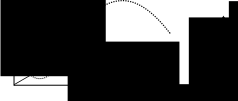
\includegraphics{./appen/rotateaxes.png}
\caption{Rotation of axes by Euler rotation $R(0\frac{\pi}{2}0)$ \label{fig:rotateaxes}.}
\end{center}
\end{figure}

For the purposes of working with the Slater-Koster parameters in 
a tightbinding Hamiltonian it remains to determine the representation of
the symmetry operation in the basis of the spherical harmonics.

The elements of the matrix representation of this symmetry operation 
can be given by $D^{l}(\Rs(0\beta0))_{m,m'}$; these are sometimes reffered to as 
the Wigner matrices. The elements of the Wigner matrix can be computed using the Euler angles
appropriate for the symmetry operation. For the example we have chosen the symmetry representation
in the basis of spherical harmonics is:
%
\begin{equation}
\left[\begin{array}{ccccc}
0  & -1 &  0 & 0 & 0 \\
1  &  0 &  0 & 0 & 0 \\
0  &  0 & -1 & 0 & 0 \\
0  &  0 &  0 & \frac{1}{2} & \frac{1}{2}\sqrt{\frac{3}{2}} \\
0  &  0 &  0 & \frac{1}{2}\sqrt{\frac{3}{2}} & \frac{1}{2}
\end{array}\right]
\end{equation}
%

\section{Rotating Slater-Koster Coefficients}
The Slater-Koster coefficients are at the heart of the tight-binding method.
The Slater-Koster table plays the role for a materials scientist that a table 
of logarithms may have for a 19th century clerk.
The table is composed of the Slater-Koster coefficients 
and the energy integrals. The latter are the matrix
elements between spherical harmonics centered on two atoms and separated
by the vector $R_a$ (see Fig.\ref{SK}). 
The coefficients in that table are expressions involving combinations 
of the direction cosines connecting the two atoms.
These arise naturally from the rotation matrices required 
to reorient the vector connecting two sites so that the two
sites are oriented purely along the axis $z$.
In this frame Slater-Koster then make a further approximation
by assuming the energy integrals can be resolved in terms
of $\sigma$, $\pi$, $\delta$ bonds. This is accomplished by writing:
%
\begin{equation}
R(\alpha\beta\gamma) \bra l_{1}m'_{1}|H|l_{2}m'_{2}\ket = R(\alpha\beta\gamma)\bra l_{1}m'_{1}|H|l_{2}m'_{2}\ket' \delta_{m'_1,m'_2}
\end{equation}
%
In the Slater-Koster two center approximation the Hamiltonian matrix 
element between two states in an arbitrary position, one relative to the other is written:
%
\begin{equation}
H_{\alpha\beta}= \sum_{m_{1}'}J(l_{1}m_{1},l_{2}m_{2}m'_{1}) \bra l_{1}m_{1}'|H|l_{2}m_{1}' \ket
\end{equation}

%Sharma's J function is equivalent to the Slater-Koster coefficients and in terms of rotation
%matrices for the spherical Harmonics is written:
%\begin{equation}
%J(l_1 m_1 l_2 m_2 m'_{1}) = D^{l_1}*_{m_1',m_1}(\alpha\beta\gamma)D^{(l_2)}_{m'_1,m_2}(\alpha\beta\gamma).
%\end{equation}

Thus when the energy integrals have been determined, by computation or interpolation,  
they can be rotated by the Slater-Koster coefficients to an arbitrary position 
in a new reference frame. This allows Hamiltonians for a variety of crystals, 
BCC, FCC, HCP, diamond etc., to be easily initialized and studied in terms of a 
local geometric picture of the electron interactions in a basis of spherical harmonics. 

\section{Derivatives of Slater-Koster Parameters}
If we choose to work in spherical coordinates centered on one atom with 
the vector between our starting atom and the target atom denoted $R_{ij}$.

The correspondence between the Cartesian system and the spherical one can be given
in the usual way:
%
\begin{align}
x = r\cos\theta\sin\phi \\
y = r\sin\theta\sin\phi \\
z = r\cos\phi
\end{align}

with the inverse map:
%
\begin{align}
r=\sqrt{x^{2}+y^{2}+z^{2}} \\
\theta = \tan^{-1}(\frac{y}{x}) \\
\phi = \cos^{-1}(\frac{z}{r})
\end{align}

We will switch between $R$ and $r$ to denote the radial coordinate but
from the context it should not raise any issues. 

One quantity of interest is the derivative of the bond integral
matrix elements in the tight binding formalism which we write
as $\nabla^{ij}_{\alpha}h^{nq}_{ij}$.

The Slater-Koster parameters are given in terms of the direction
cosines of the vector connecting the two atoms $R_{ij}$ written
$l,m,n$. These direction cosines can enter the Slater-Koster expressions
linearly, as squares, or to the fourth power.

In spherical coordinates the gradient can be written:
%
\begin{equation}
\nabla =  \hat{r} \frac{\partial}{\partial r} 
          + \frac{1}{r}\hat{\phi}\frac{\partial}{\partial\phi}
          + \frac{1}{r\sin\phi}\hat{\theta}\frac{\partial}{\partial \theta}
\end{equation}

It is also useful to have the Cartesian partial derivatives written in spherical
coordinates for reference:

\begin{flalign}
\label{eq:cartpartials}
\frac{\partial}{\partial x}  =& \cos\theta\sin\phi\frac{\partial}{\partial r}
                             - \frac{\sin\theta}{r\sin\phi}\frac{\partial}{\partial \theta}
                             + \frac{\cos\theta\cos\phi}{r}\frac{\partial}{\partial \phi}\\
\frac{\partial}{\partial y}  =& \sin\theta\sin\phi\frac{\partial}{\partial r}
                             + \frac{\cos\theta}{r\sin\phi} \frac{\partial}{\partial \theta}
                             + \frac{\sin\theta\cos\phi}{r} \frac{\partial}{\partial \phi}\\
\frac{\partial}{\partial z}  =& \cos\phi\frac{\partial}{\partial r}
                             - \frac{\sin\phi}{r}\frac{\partial}{\partial\phi}
\end{flalign}

\section{Two Center Derivatives of Bond Integrals}
We will assume in what follows a scaling of the energy integrals 
as the inverse fifth power of the distance between the atoms.
The precise functional form chosen for this decay does not change
the principles of the following derivation.

We may write the integrals:
%
\begin{equation}
h^{rs}_{ij} = \frac{f_{rs}(l,m,n)}{R_{ij}^{5}}
\end{equation}
where $rs$ is the combination of spherical harmonics and $ij$ are the atom sites.
Let us look at how this energy integral varies with a perturbation of atom $i$ along $x$.
We can choose a couple different coordinate systems to take the derivative efficiently.
One way to do it is convert all the direction cosines into cartesian coordinates.

The partial derivative with respect to $\alpha = x,y,z$ are then:
%
\begin{equation}
\label{eq:derivSK}
\frac{\partial h^{rs}_{ij}}{\partial \alpha} = (\frac{-5}{R^{6}})(\frac{\partial R}{\partial \alpha})f^{rs}(l,m,n) 
                                             + \frac{1}{R^{5}}\frac{\partial f^{rs}(l,m,n)}{\partial \alpha}
\end{equation}
%
where f(l,m,n) is the Slater-Koster integral for the orbital combination $rs$.
The derivate of $R$ w.r.t to $x$ gives the direction cosine $l=x/R$ so the first contribution to the 
derivative is just the direction cosine for $x$, i.e. $l$, multiplied by 
the standard Slater-Koster term and weighted by the radial decay. 
The second term is the derivative of the Slater-Koster term with 
respect to a cartesian coordinate. This can be handled using the chain rule:
%
\begin{equation}
\frac{\partial f^{rs}(l,m,n)}{\partial x} = \frac{df^{rs}(l,m,n)}{dl}\frac{dl}{dx}
\end{equation}
%

NB the variation of the other direction cosines, $m,n$, w.r.t. $l$, and 
$l$ w.r.t. $x$: 
%
\begin{align}
\frac{dm}{dl} = \frac{-ml}{(1-l^2)} \\
\frac{dn}{dl} = \frac{-nl}{(1-l^2)} \\
\frac{dl}{dx} = \frac{(1-l^{2})}{R}
\end{align}
%
These terms contribute additional terms to the derivatives of the 
two center Slater-Koster terms. Eq.~\ref{eq:derivSK} then 
gives the first order variation of the matrix elements for
an $~R^{-5}$ dependence of the hopping integrals.

\subsubsection{Example: $h^{xy,yz}$ }
Let us take the Slater-Koster coefficient for $h^{xy,yz}$. 
We can write this overlap integral in terms of the two center bond integrals 
and the direction cosines as (after a slight rearrangement from the original table):
% 
\begin{equation}
h^{xy,yz} = \frac{ln(dd\pi-dd\delta) + lm^{2}n (3dd\sigma-4dd\pi+dd\delta)}{R^5}
\end{equation}
%

The angular part (i.e. the contribution to the derivative from the first order variation in 
the Slater-Koster coefficients w.r.t. $l$) is:

\begin{equation}
\frac{d{f^{xy,yz}(lmn)}}{dl} = (n + \frac{dn}{dl})(dd\pi-dd\delta) 
                                                  + (m^{2}n +2lmn\frac{dm}{dl}+lm^{2}\frac{dn}{dl})(3dd\sigma-4dd\pi+dd\delta)
\end{equation}

Adding the radial contribution gives the total partial derivative with respect to a cartesian coordinate:
%
\begin{equation}
\frac{\partial h^{xy,yz}_{ij}}{\partial x} =  \frac{1}{R^{6}}[-5lf^{xy,yz}(l,m,n) + (1-l^{2})\frac{df^{xy,yz}(l,m,n)}{dl}]
\end{equation}
%

\subsection{Exponential Decay}
As physicists, or materials scientists, it is permitted, perhaps too often permitted, to skip formal
justification and generality and just pick functions that are simple to work with. In all honesty this
is the reason the power law decay is chosen and the same motivation underlies the choice of exponential
decay. There are justifications and appeals to utility but the simple fact is the function can be written
down, it's derivatives are straight forward, and it decays. 

In the case of the decay of the radial integrals being exponential:
we can write:
%
\begin{equation}
\frac{\partial h^{rs}_{ij}}{\partial \alpha} = e^{-q|R|}(-q(\frac{\partial R}{\partial \alpha})f(l,m,n) + 
\frac{\partial f(l,m,n)}{\partial l}\frac{\partial l}{\partial alpha})
\end{equation}

\section{A Menagerie of Tight Binding Parameters}
%The parameters used in Ref.~\cite{burke78} are appropriate to the BCC structure.
%The tightbinding Hamiltonian only considers two center contributions, with the parameters 
%coming from Pettifor\cite{pettifor69} and rescaled to produce the observed
%bandwidth of tungsten. The parameters are given in Table~\ref{tab:dsurface}.
For ease of reference we collect here d tight-binding coefficicents
that have found there way into the literature. The choice of these parameters
is very much an example of theoretical materials science constituting a 
craft. In later chapters we will examine some of the developments that set
tight-binding and the choice of coefficients on a more definite 
theoretical framework. The Slater-Koster parameters used for FCC, BCC, 
and HCP crystals in Ref.~\cite{haydock72} are given in Table \ref{tab:pettiparams}.
%
\begin{table}
\begin{center}
\begin{tabular}{|c|c|c|c|c|} 
\hline
Structure & $dd\sigma$ & $dd\pi$  & $dd\delta$ &  Band-limits \\
\hline
FCC       & -0.027784  & 0.012535 & -0.001554  & -0.131 to 0.085 \\ 
\hline
HCP       & -0.027784  & 0.012535 & -0.001554  & -0.119 to 0.081 \\
\hline
BCC       & -0.03248   & 0.01538  & -0.00200   & -0.119 to 0.097 \\
          & -0.01341   & 0.00487  & -0.00049   &              \\
\hline
\end{tabular}
\caption{Slater-Koster parameters from Pettifor \cite{pettifor69}, 
along with band edges in Ry. First and second nearest neighbour 
parameters are given for BCC crystals. \label{tab:pettiparams}.}
\end{center}
\end{table}
%
%\begin{table}
%\begin{tabular}{|c|c|c|}
%\hline
%SK Parameter & First Neighbour & Second Nearest Neighbour \\
%\hline
%$dd\sigma$ & -0.02992  & -0.05364 \\
%$dd\pi$    &  0.06652  &  0.01943 \\
%$dd\delta$ &  0.00800  &  0.00196 \\
%\hline
%\end{tabular}
%\caption{These parameters are difficult to make out from the electronic version of Ref.
%due to poor resolution of the scan. \label{tab:dsurface}.}
%\end{table}
%
\begin{table}
\begin{center}
\begin{tabular}{|c|c|c|}
\hline
\multicolumn{3}{|c|} {FCC TB Parameters} \\
\hline
Integral & 1st Nearest Neighbour & 2nd Nearest Neighbours \\
\hline
$dd\sigma$ & -0.027784 & - \\
$dd\pi$    &  0.012535 & - \\
$dd\delta$ & -0.001554 & - \\
\hline
\multicolumn{3}{|c|} {BCC TB Parameters} \\
\hline
Integral & 1st Nearest Neighbour & 2nd Nearest Neighbours \\
$dd\sigma$ & -0.06560  & -0.03195 \\
$dd\pi$    &  0.04373  & 0.02130\\
$dd\delta$ & -0.010934 & -0.00537\\
\hline
\end{tabular}
\caption{The tight binding parameters used for the example recursion 
calculations in this chapter, in the FCC lattice only nearest neighbours 
are included.}
\end{center}
\end{table}

Whether we are able to create a tight binding description of transition metals
depends on whether a decent, energy independent, approximation to the electronic 
structure in fcc/bcc metals can be achieved with 9x9 matrices describing 
nearest neighbour interactions of spherical harmonics or Wannier functions 
in the Slater-Koster form.



The determination of the integration constants is a problem unto itself.
Tight binding parameters for the transition metals can be extracted from 
a number of places: tight binding parameters that span the transition
metal range can be found in Refs. \cite{nieminen76}, \cite{pettifor77} 
and \cite{jepsen75, andersen77, harrison80}.
Harrison has also published a set of universal parameters for s-p bonded structures.
In Chapters~\ref{chap:gw}~and~\ref{chap:wannier} we will show how 
these parameters may be obtained from first principles. 


